\uuid{JDkE}
\exo7id{5530}
\titre{exo7 5530}
\auteur{rouget}
\organisation{exo7}
\datecreate{2010-07-15}
\isIndication{false}
\isCorrection{true}
\chapitre{Courbes planes}
\sousChapitre{Coordonnées polaires}
\module{Géométrie}
\niveau{L2}
\difficulte{}

\contenu{
\texte{
Construire les courbes suivantes~:
}
\begin{enumerate}
    \item \question{$r=\sqrt{\cos(2\theta)}$,}
\reponse{(\textbf{Lemniscate de } \textsc{Bernoulli}.) Soit $\mathcal{C}$ la courbe d'équation polaire $r=\sqrt{\cos(2\theta)}$.
\textbf{Domaine d'étude.} Notons $D$ le domaine de définition de la fonction $r~:~\theta\mapsto\sqrt{\cos(2\theta)}$.
\textbullet~$\theta\in D\Leftrightarrow\theta+2\pi\in D$ et pour $\theta\in D$, 

\begin{center}
$M(\theta+2\pi)=\left[r(\theta+2\pi),\theta+2\pi\right]=\left[r(\theta),\theta+2\pi\right]=\left[r(\theta),\theta\right]=M(\theta)$.
\end{center}
On obtient donc la courbe complète quand $\theta$ décrit un intervalle de longueur $2\pi$ comme $[-\pi,\pi]$.
\textbullet~$\theta\in D\Leftrightarrow-\theta\in D$ et pour $\theta\in D$, 

\begin{center}
$M(-\theta)=\left[r(-\theta),-\theta\right]=\left[r(\theta),-\theta\right]=s_{(Ox)}(M(\theta))$.
\end{center} On étudie et on construit la portion de courbe correspondant à $\theta\in[0,\pi]$ puis on obtient la courbe complète par réflexion d'axe $(Ox)$.
\textbullet~$\theta\in D\Leftrightarrow\pi-\theta\in D$ et pour $\theta\in D$, 

\begin{center}
$M(\pi-\theta)=\left[r(\pi-\theta),\pi-\theta\right]=\left[r(\theta),\pi-\theta\right]=s_{(Oy)}(M(\theta))$.
\end{center} On étudie et on construit la portion de courbe correspondant à $\theta\in\left[0,\frac{\pi}{2}\right]$ puis on obtient la courbe complète par réflexion d'axe $(Oy)$ puis d'axe $(Ox)$.
Pour $\theta\in\left[0,\frac{\pi}{2}\right]$, $\theta\in D\Leftrightarrow\cos\left(2\theta\right)\geqslant0\Leftrightarrow\theta\in\left[0,\frac{\pi}{4}\right]$. On étudie donc la courbe sur $\left[0,\frac{\pi}{4}\right]$.
\textbf{Variations et signe de $r$.} La fonction $r$ est strictement décroissante sur $\left[0,\frac{\pi}{4}\right]$, strictement positive sur $\left]0,\frac{\pi}{4}\right]$ et s'annule en $\frac{\pi}{4}$.
\textbf{Etude en $\frac{\pi}{4}$.} $M\left(\frac{\pi}{4}\right)=O$ et donc la tangente en $M\left(\frac{\pi}{4}\right)$ est la droite passant par $O$ et d'angle polaire $\frac{\pi}{4}$ ou encore la droite d'équation $y=x$.

\textbf{Etude en $0$.} $M(0)$ est le point de coordonnées cartésiennes $(1,0)$. Pour $\theta\in\left]-\frac{\pi}{4},\frac{\pi}{4}\right[$,

\begin{center}
$\overrightarrow{\frac{dM}{d\theta}}(\theta)=-\frac{\sin(2\theta)}{\sqrt{\cos(2\theta)}}\overrightarrow{u}_\theta+\sqrt{\cos(2\theta)}\overrightarrow{v}_\theta$ et donc $\overrightarrow{\frac{dM}{d\theta}}(0)=\overrightarrow{v}_0=\overrightarrow{j}$.
\end{center}
$M(0)$ est le point de coordonnées cartésiennes $(1,0)$ et la tangente en $M(0)$ est dirigée par $\overrightarrow{j}$

$$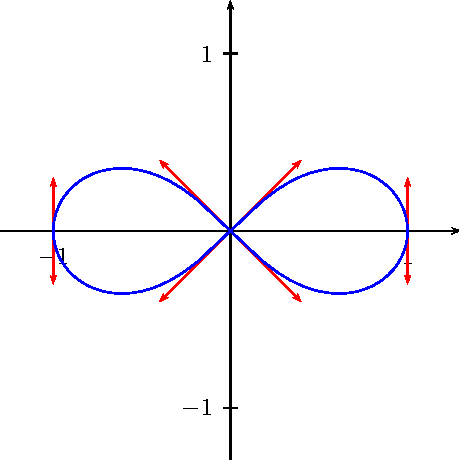
\includegraphics{../images/pdf/JDkE-1.pdf}$$}
    \item \question{$r=\sin\left(\frac{2\theta}{3}\right)$,}
\reponse{Soit $\mathcal{C}$ la courbe d'équation polaire $r=\sin\left(\frac{2\theta}{3}\right)$.
\textbf{Domaine d'étude.} \textbullet~Pour $\theta\in \Rr$, 

\begin{center}
$M(\theta+6\pi)=\left[r(\theta+6\pi),\theta+6\pi\right]=\left[r(\theta),\theta+6\pi\right]=\left[r(\theta),\theta\right]=M(\theta)$.
\end{center}
On obtient donc la courbe complète quand $\theta$ décrit un intervalle de longueur $6\pi$ comme $[-3\pi,3\pi]$.
\textbullet~Pour $\theta\in[-3\pi,3\pi]$, 

\begin{center}
$M(-\theta)=\left[r(-\theta),-\theta\right]=\left[-r(\theta),-\theta\right]=\left[r(\theta),\pi-\theta\right]=s_{(Oy)}(M(\theta))$.
\end{center} 
On étudie et on construit la portion de courbe correspondant à $\theta\in[0,3\pi]$ puis on obtient la courbe complète par réflexion d'axe $(Oy)$.
\textbullet~Pour $\theta\in[0,3\pi]$, $M(3\pi-\theta)=\left[r(3\pi-\theta),3\pi-\theta\right]=\left[-r(\theta),3\pi-\theta\right]=\left[r(\theta),-\theta\right]=s_{(Ox)}(M(\theta))$.
 On étudie et on construit la portion de courbe correspondant à $\theta\in\left[0,\frac{3\pi}{2}\right]$ puis on obtient la courbe complète par réflexion d'axe $(Ox)$ puis d'axe $(Oy)$.
 
 
\textbullet~Pour $\theta\in\left[0,\frac{3\pi}{2}\right]$, $M\left(\frac{3\pi}{2}-\theta\right)=\left[r\left(\frac{3\pi}{2}-\theta\right),\frac{3\pi}{2}-\theta\right]=\left[r(\theta),\frac{3\pi}{2}-\theta\right]=s_{y=-x}(M(\theta))$.
 On étudie et on construit la portion de courbe correspondant à $\theta\in\left[0,\frac{3\pi}{4}\right]$ puis on obtient la courbe complète par réflexions successives d'axes la droite d'équation $y=-x$, puis d'axe $(Ox)$ et enfin d'axe $(Oy)$.
 
 
\textbullet~\textbf{Remarque.} La fonction $r$ admet $3\pi$ pour plus petite période strictement positive. Pourtant, on n'obtient pas la courbe complète quand $\theta$ décrit $[0,3\pi]$ car $3\pi$ ne fournit pas un nombre entier de tours. Plus précisément,

\begin{center}
$M(\theta+3\pi)=\left[r(\theta+3\pi),\theta+3\pi\right]=\left[r(\theta),\theta+\pi\right]=s_O(M(\theta))$.
\end{center}

\textbf{Variations et signe de $r$.} La fonction $r$ est strictement positive sur $\left]0,\frac{3\pi}{4}\right]$ et s'annule en $0$. La fonction $r$ est strictement croissante sur $\left[0,\frac{3\pi}{4}\right]$.
\textbullet~$M(0)$ est le point $O$. La tangente en $M(0)$ est la droite passant par $O$ d'angle polaire $0$ c'est-à-dire l'axe $(Ox)$.

$$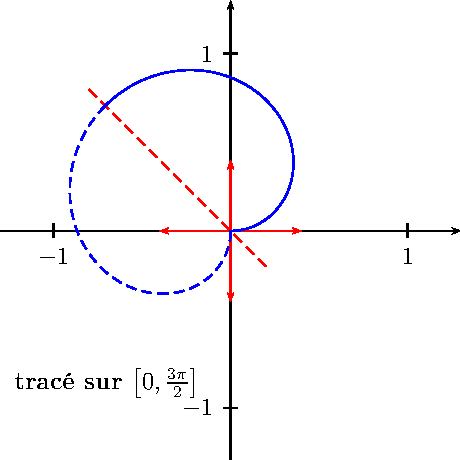
\includegraphics{../images/pdf/JDkE-2.pdf}$$

$$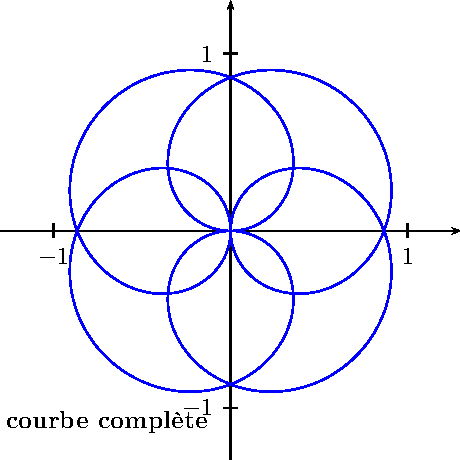
\includegraphics{../images/pdf/JDkE-3.pdf}$$}
    \item \question{$r=ae^{b\theta},\;(a,b)\in]0,+\infty[^2$,}
\reponse{Soit $\mathcal{C}$ la courbe d'équation polaire $r=ae^{b\theta}$.
L'étude est très brève. La fonction $r~:~\theta\mapsto ae^{b\theta}$ est strictement positive et strictement croissante sur $\Rr$. Tout en tournant, on ne cesse de s'écarter de l'origine~:~la courbe est une spirale.

$$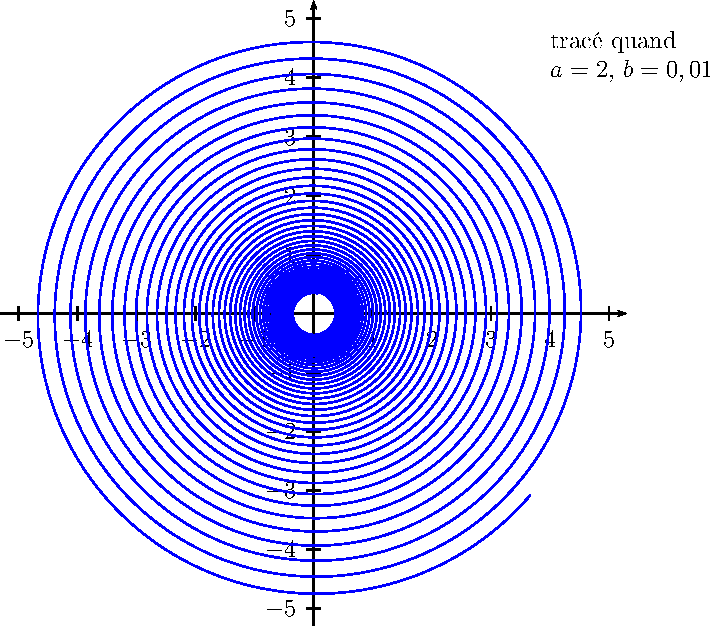
\includegraphics{../images/pdf/JDkE-4.pdf}$$}
    \item \question{$r=2\cos(2\theta)+1$,}
\reponse{Soit $\mathcal{C}$ la courbe d'équation polaire $r=2\cos(\theta)+1$.

\textbf{Domaine d'étude.} \textbullet~Pour $\theta\in \Rr$, $M(\theta+2\pi)=M(\theta)$. On obtient donc la courbe complète quand $\theta$ décrit un intervalle de longueur $2\pi$ comme $[-\pi,\pi]$.
\textbullet~Pour $\theta\in[-\pi,\pi]$, $M(-\theta)=s_{(Ox)}(M(\theta))$. On étudie et on construit la portion de courbe correspondant à $\theta\in[0,\pi]$ puis on obtient la courbe complète par réflexion d'axe $(Ox)$.
\textbf{Variations et signe de $r$.} La fonction $r$ est strictement décroissante sur $[0,\pi]$. La fonction $r$ est strictement positive sur $\left[0,\frac{2\pi}{3}\right[$, strictement négative sur $\left]\frac{2\pi}{3},0\right]$ et s'annule en $\frac{2\pi}{3}$. Donc la fonction $\theta\mapsto OM(\theta)=|r(\theta)|$ est strictement décroissante sur $\left[0,\frac{2\pi}{3}\right]$ et strictement croissante sur $\left[\frac{2\pi}{3},\pi\right]$.
\textbullet~$M\left(\frac{2\pi}{3}\right)$ est le point $O$. La tangente en $M\left(\frac{2\pi}{3}\right)$ est la droite passant par $O$ d'angle polaire $\frac{2\pi}{3}$ c'est-à-dire la droite d'équation $y=-\sqrt{3}x$.
\textbullet~Par symétrie par rapport à $(Ox)$, les tangentes en $M(0)$ et $M(\pi)$ sont parrallèles à $(Oy)$.

$$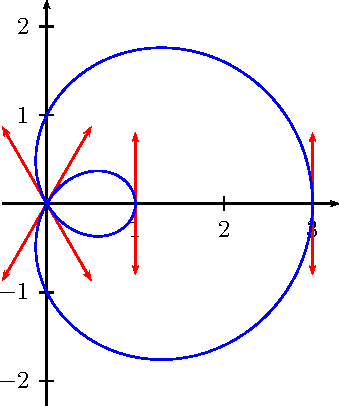
\includegraphics{../images/pdf/JDkE-5.pdf}$$}
    \item \question{$r=\tan\left(\frac{2\theta}{3}\right)$.}
\reponse{Soit $\mathcal{C}$ la courbe d'équation polaire $r=\tan\left(\frac{2\theta}{3}\right)$.
\textbf{Domaine d'étude.}  Notons $D$ le domaine de définition de la fonction $r~:~\theta\mapsto\tan\left(\frac{2\theta}{3}\right)$.
\textbullet~$\theta\in D\Leftrightarrow\theta+6\pi\in D$ et $M(\theta+6\pi)=M(\theta)$. On obtient donc la courbe complète quand $\theta$ décrit un intervalle de longueur $6\pi$ comme $[-3\pi,3\pi]$.
\textbullet~$\theta\in D\Leftrightarrow -\theta\in D$ et $M(-\theta)=s_{(Oy)}(M(\theta))$. On étudie et on construit la portion de courbe correspondant à $\theta\in[0,3\pi]$ puis on obtient la courbe complète par réflexion d'axe $(Oy)$.
\textbullet~$\theta\in D\Leftrightarrow 3\pi-\theta\in D$ et $M(3\pi-\theta)=s_{(Ox)}(M(\theta))$. On étudie et on construit la portion de courbe correspondant à $\theta\in\left[0,\frac{3\pi}{2}\right]$ puis on obtient la courbe complète par réflexion d'axe $(Ox)$ puis par réflexion d'axe $(Oy)$.
\textbullet~$\theta\in D\Leftrightarrow \frac{3\pi}{2}-\theta\in D$ et 

\begin{center}
$M\left(\frac{3\pi}{2}-\theta\right)=\left[-r(\theta),\frac{3\pi}{2}-\theta\right]=\left[r(\theta),\frac{\pi}{2}-\theta\right]=s_{y=x}(M(\theta))$.
\end{center}
On étudie et on construit la portion de courbe correspondant à $\theta\in\left[0,\frac{3\pi}{4}\right]$ puis on obtient la courbe complète par réflexions successives d'axe la droite d'équation $y=x$, puis d'axe $(Ox)$ et enfin d'axe $(Oy)$.
\textbullet~Pour $\theta\in\left[0,\frac{3\pi}{4}\right]$, $r(\theta)$ existe si et seulement si $\theta\neq\frac{3\pi}{4}$. On étudie donc sur $\theta\in\left[0,\frac{3\pi}{4}\right[$.

\textbf{Variations et signe de $r$.} La fonction $r$ est strictement croissante sur $\left[0,\frac{3\pi}{4}\right[$, strictement positive sur $\left]0,\frac{3\pi}{4}\right[$ et s'annule en $0$.

\textbullet~La tangente en $M(0)=O$ est la droite passant par $O$ et d'angle polaire $0$ c'est-à-dire l'axe $(Ox)$.
\textbullet~\textbf{Etude quand $\theta$ tend vers $\frac{3\pi}{4}$.} Quand $\theta$ tend vers $\frac{3\pi}{4}$ par valeurs inférieures, $r(\theta)$ tend vers $+\infty$. la courbe admet donc une direction asymptotique d'angle polaire $\frac{3\pi}{4}$ ou encore d'équation $y=-x$.
Recherchons une éventuelle droite asymptote. Pour cela, étudions $\displaystyle\lim_{\substack{\theta\rightarrow\frac{3\pi}{4}\\ \theta<\frac{3\pi}{4}}}r(\theta)\sin\left(\theta-\frac{3\pi}{4}\right)$. Posons $h=\frac{3\pi}{4}-\theta$ ou encore $\theta=\frac{3\pi}{4}-h$.
\begin{center}
$r(\theta)\sin\left(\theta-\frac{3\pi}{4}\right)=\tan\left(\frac{\pi}{2}-\frac{2h}{3}\right)\sin(-h)=-\cotan h\sin h=-\cos h\rightarrow-1$.
\end{center}
Ainsi, $\mathcal{C}$ admet une droite asymptote $(D)$ quand $\theta$ tend vers $\frac{3\pi}{4}$. De plus,

\begin{center}
$M(x,y)\in(D)\Leftrightarrow\overrightarrow{OM}.\overrightarrow{v}_{\frac{3\pi}{4}}=-1\Leftrightarrow-\frac{1}{\sqrt{2}}x-\frac{1}{\sqrt{2}}y=-1\Leftrightarrow y=-x+\sqrt{2}$.
\end{center}

$$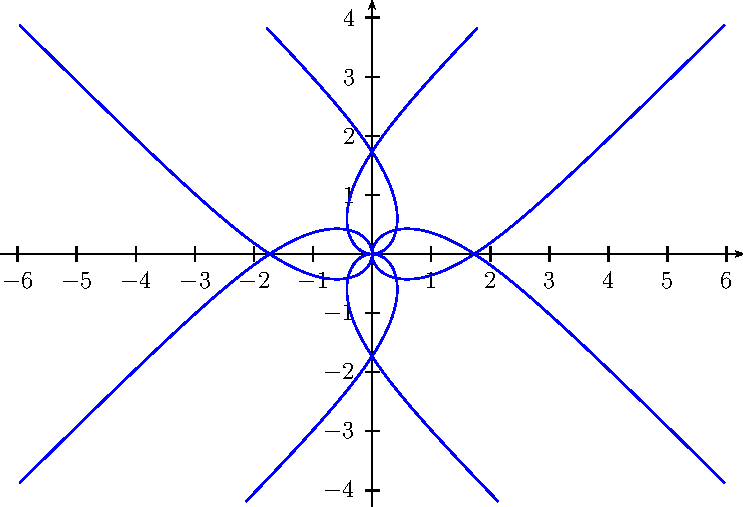
\includegraphics{../images/pdf/JDkE-6.pdf}$$}
\end{enumerate}
}
